\section{Prompt Design for Graph Tasks}\label{sec:ptask}
In this section, we propose a unified view for the graph prompt. As shown in \figref{fig:prompt}, the graph prompt should contain at least three components: prompt tokens with prompt vector; token structures preserving inner correlations of these tokens; and inserting patterns indicating how to integrate the original graph with prompts. Beyond these details, we are particularly interested in the following questions: \textit{Question 1:} How do these works design the graph prompt? \textit{Question 2:} How do these works reformulate downstream tasks to the pre-training tasks? \textit{Question 3:} How do these works learn an effective prompt? and \textit{Question 4:} What are the inner connections of these works, their advantages and limitations? With these questions, we summarize the most representative works published recently and present them in \tabref{tab:graph_prompt_summary}.


\begin{figure}[t]
    \centering
    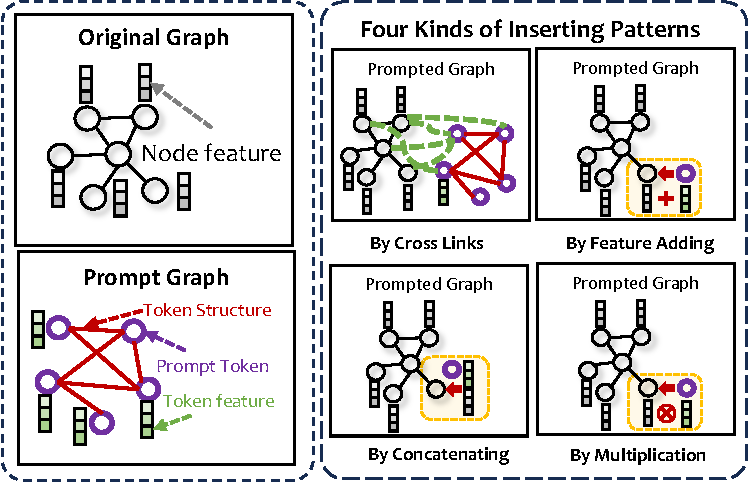
\includegraphics[width=0.49\textwidth]{pic/prompt.pdf}
    \caption{Prompt Tokens, Structures, and Inserting Patterns.}
    \label{fig:prompt}
\end{figure}



\subsection{Prompt Token, Structure, and Inserting Pattern}\label{subsec:pdesign}

\textit{\dotuline{Question 1: How do They Design A Graph Prompt?}}

\textbf{A. Prompt as Tokens. }
The simplest graph prompt can be treated as some additional features added to the original graph features \cite{zhu2023graphcontrol}. For example, given a graph feature matrix $\mathbf{X}=\{x_1,\cdots, x_N\} \in \mathbb{R}^{N\times d}$ where $x_i\in \mathbb{R}^{1\times d}$ is the feature of $i$-th node and $d$ is the dimension of the feature space. \citet{fang2022prompt} and \citet{shirkavand2023deep} treat the basic prompt as a learnable vector $p \in \mathbb{R}^{1\times d}$, which can be added to all node features and make the manipulated feature matrix be $\mathbf{X}^{*}=\{x_1+p,\cdots, x_N+p\}$. In this way, we can use the reformulated features to replace the original features and process the graph with pre-trained graph models. A later work \cite{fang2023universal} further extends one prompt token to multiple tokens and makes the performance better. PGCL \cite{gong2023prompt} design a prompt vector for semantic view and another prompt vector for contextual view, then they add these prompt vectors to the graph-level representations by element-wise multiplication. A similar prompt design is also adopted in VNT \cite{tan2023virtual}. The difference is that their inserting pattern does not add the prompt token to the original graph feature but concatenates the prompt token with the original node set and tries to integrate them by the self-attention function in a graph transformer. In GraphPrompt \cite{liu2023graphprompt}, the prompt token is similar to the format defined by \citet{fang2022prompt}. The difference thing is that previous work designed the prompt tokens in the initial feature space, while this method assumes the prompt in the hidden layer of the graph model. Usually, the hidden size will be smaller than the original feature, making their prompt token shorter than the previous one. Another different thing is that the graph prompt here is used to assist graph pooling operation (a.k.a $\text{Readout}$). For example, given the node set $\mathcal{V}=\{v_1,\cdots, v_{|\mathcal{V}|}\}$, the embedding of node $v$ is $\textbf{h}_v \in \mathbb{R}^{1\times d}$, a prompt token $\textbf{p}_t \in \mathbb{R}^{1\times d}$ specified to task $t$ is inserted to the graph nodes by the element-wise multiplication ($\otimes$): $\textbf{s}_t=\text{Readout}(\{\textbf{p}_t \otimes \textbf{h}_v:v \in \mathcal{V}\})$. Similarly, SGL-PT \cite{zhu2023sglpt} creates a prompt token to connect to all nodes in the graph. The prompt token preserves a global perception of the graph and can assist their global branch of the pre-training tasks, which can be also treated as a pooling strategy. Aiming at aligning node classification and link prediction, GPPT \cite{sun2022gppt} defines graph prompts as additional tokens that contain task tokens and structure tokens. Here the task token refers to the description of the downstream node label to be classified and the structure token is the representation of the subgraph surrounding the target node. By this means, predicting node $v$'s label can be reformulated to predict a potential link between node $v$'s structure token and the label task token. 
Aiming at the node classification task, ULTRA-DP \cite{chen2023ultradp} creates a prompt token for each target node, where the token feature is the weighted sum of position embedding of the target node and a task embedding of the pre-training task. HetGPT \cite{ma2023hetgpt} design a prompt with node tokens and class tokens, which are organized in a similar way to GPPT. The difference is that they also add a type-specific feature token to make graph prompts sensitive to different node types, by which they can extend existing graph prompts to heterogeneous graphs. 




\textbf{B. Prompt as Graphs. }
The graph prompt in All in One \cite{sun2023all} is an additional subgraph that can be learned by efficient tuning. The prompt tokens are some additional nodes that have the same size of node representation as the original nodes. They assume the prompt tokens should be in the same semantic space as the original node features so that we can easily manipulate node features with these tokens. The token structures include two parts. The first part is the inner links among different tokens, and the second part is the cross-links between the prompt graph and the original graph. These links can be pre-calculated by the dot product between one token to another token (inner links) or one token to another original node (cross links). The inserting pattern is to add the prompt graph to the original graph by the cross-links and then treat the combined graph as a new graph, and send it to the pre-trained graph model to get the graph-level representation. The prompt graph in PRODIGY \cite{huang2023prodigy} includes data graphs and a task graph. The data graphs can be treated as subgraphs surrounding the target nodes (for node classification task), node pairs (for edge classification task), or just denoted as the graph classification instance. Here the prompt tokens and prompt structures are just the same as in the original graph. The task graph contains data tokens and label tokens where each data token connects to one data graph and is further connected by label tokens. Unlike previous works that aim at reformulating downstream tasks to the pre-training task by prompting the downstream data, PRODIGY leverages the prompt graph to unify all the upstream and downstream tasks. Their pre-training strategy is a set of tasks including neighboring matching and label matching, which can be reformulated as predicting the similarity between the data token and the label token in the prompt graph. SAP \cite{ge2023enhancing} also connects several prompt tokens (each token corresponds to one class) to the original graph by cross-links defined in All in One. The difference is that their prompting task is a node-level contrastive task, in which they use MLP to encode the node features as the first view and they use a GNN to encode the prompted graph as the second view, which is consistent with their pre-training task.


\subsection{Aligning Tasks by Answering Function}\label{subsec:align}

\textit{\dotuline{Question 2: How do they reformulate downstream tasks to the pretext?} }

\textbf{A. Handling Different Level Tasks.} 
All in One \cite{sun2023all} pre-trains the graph model via graph-level contrastive learning. The pre-training task aims to learn a robust graph encoder over different graph views generated by the perturbations of the original graph. To reformulate various graph tasks to this graph-level pretext, they first unify node-level, edge-level, and graph-level tasks to the graph-level task by induced subgraphs, which are also introduced in PRODIGY \cite{huang2023prodigy,liu2023graphprompt,gong2023prompt}. Then they claim that the graph prompt added to the original graph is in nature the simulation of any graph operations such as node feature masking, node or edge perturbations, subgraph removing, etc. With this opinion, we just need to add an appropriate graph prompt to downstream graph datasets then it will be promising to further reformulate the downstream task to the pretext. 


\textbf{B. Learnable Answering Function.} 
To output the results of downstream tasks, \citet{sun2023all} design two types of answering functions. The first one is a learnable task head (such as an MLP mapping function) that can be easily tuned with very limited data. It takes the graph-level representation generated by the pre-trained graph model and then outputs the downstream result. For example, if the downstream is a three-class node classification, we can simply use a dense layer with three hidden units to connect the graph representation, which is generated by the pre-trained model on the combined graph with node included graph and a graph prompt. In this case, both the graph prompt and the task head are tunable, so we can adjust them alternately. Similar learnable answering functions are also adopted in other works like \cite{fang2022prompt, fang2023universal,tan2023virtual}. The good point is that they are very easy to align two tasks, however, it also increases the tuning workflow. 



\textbf{C. Hand-crafted Answering Function.} 
To further reduce the tuning burden, All in One \cite{sun2023all} also proposes a second answering function, which is hand-crafted without any trainable task head. For example, for a node classification task, we can set up $K$ unique sub-prompts, each aligning with a different node type, where $K$ represents the total number of node categories. If the pre-training involves a task like GraphCL \cite{you2020graph}, which aims to maximize similarity at the graph level between pairs of graph views, then the target node can be classified with label $\ell, (\ell=1,2,\cdots,K)$ if the $\ell$-th graph most closely resembles the original node-inclusive graph. Similarly, GPPT \cite{sun2022gppt} and  HetGPT \cite{ma2023hetgpt} use link prediction as their pre-training task and reformulate downstream node classification by unifying it as the same task template. For example, by treating the node label as an additional token, we can use the pre-trained model to directly output the possibility of an edge between the label token and the target node. 
The pre-training strategy in SAP \cite{ge2023enhancing} is to compare node representations from two graph views, the first of which is generated by node feature encoding and the second of which is encoded by a graph model. To this end, their prompt tokens denote class information and they compare node representation with each class token to find the class with the largest similarity as the inference results. By designing a unified task template, PRODIGY \cite{huang2023prodigy} uses a hand-crafted graph prompt to describe all node, edge, and graph classification tasks by predicting the link between data tokens and label tokens. \citet{liu2023graphprompt} extend the link prediction task as graph pair similarity and treat it as their pre-training task, to align the downstream node classification and graph classification task, they design a unified answering template making the downstream side aligned with the pre-training side. Specifically, given a triplet of induced graphs $(g_1,g_2, g_3)$ where $g_1$ and $g_2$ have the same label, $g_1$ and $g_3$ have different labels. In particular, when the target task is node classification, the induced graph refers to the contextual subgraph of the target node. The unified answering template is defined as  $\text{sim}(g_1,g_2)>\text{sim}(g_1,g_3)$.



\subsection{Prompt Tuning}\label{subsec:pt}

\textit{\dotuline{Question 3: How do They Learn A Graph Prompt? }}

\textbf{A. Meta-Learning Technique. }
To learn appropriate prompts, \citet{sun2023all}  leverage meta-learning techniques (such as MAML\cite{finn2017modelagnostic} model) to obtain a robust starting point for the prompt parameters. Since the support set and query set include various graph tasks (such as node classification, link prediction, graph classification, etc), the learned graph prompt is expected to be more general on various downstream tasks. 

\textbf{B. Task-specific Tuning. }
Besides All in One \cite{sun2023all}, which aims to learn a general prompt on various downstream tasks, there are also some works that target specific downstream tasks such as graph classification. In this case, the prompt tuning can be more task-directed. For example, GPF \cite{fang2022prompt} aims at a graph classification task, so it just needs to tune the prompt token $\textbf{p}$ and the task head $\phi$ by maximizing the likelihood of predicted correct graph labels given the prompted graph representation $\tilde{\textbf{s}}_i$ from the pre-trained graph model $\pi$. In this case, the task head tuning and the prompt tuning share the same objectives, which can be formulated by: $\max_{\textbf{p}, \phi} \sum_{(y_i,\tilde{\textbf{s}}_i)} p_{\pi, \phi} (y_i| \tilde{\textbf{s}}_i)$.



\textbf{C. Tuning in Line with Pretext. }
Intuitively, prompting aims at reformulating downstream tasks to the pre-training task. Therefore, it would be more natural if the prompt tuning shares the same objective with the pre-training task. As suggested in GraphPrompt \cite{liu2023graphprompt}, the authors use a similar loss function to learn prompts. Similarly, GPPT \cite{sun2022gppt} and VNT \cite{tan2023virtual} adopt the same loss function (Cross-Entropy) as their link prediction and node classification tasks, respectively. HetGPT \cite{ma2023hetgpt} and  SAP \cite{ge2023enhancing} use a node-level contrastive loss to learn their prompt tokens because their pre-training task is also conducted by the same contrastive task (node pair comparison). PGCL \cite{gong2023prompt} introduces graph-level loss to align with the pre-training task. ULTRA-DP \cite{chen2023ultradp} develop two pre-training tasks including edge prediction and neighboring prediction, each of which corresponds to one task embedding. In the pre-training phase, they randomly select a task and then integrate specific task-related embeddings into the prompt tokens. These learnable task embeddings are then trained with the graph model. 



\subsection{Further Discussion}\label{subsec:pdiscussion}

\textit{\dotuline{Question 4: What are Their Connections, Pros and Cons?}}

The good point of GPF \cite{fang2022prompt} is that they propose a very simple prompt that can be easily used in various pre-training tasks and downstream tasks. However, a single prompt token added to all nodes is very limited in expressiveness and generalization. A potential solution is to learn an independent prompt token for each node, which means one node corresponds to one prompt token, but this will cause low efficiency in parameters. To this end, we can train K-independent basis vectors and use them to compound each node token (GPF-Plus \cite{fang2023universal}). This improvement makes their work have more similar insights with All in One \cite{sun2023all}.


HetGPT \cite{ma2023hetgpt} extends prompt tokens to type-specific format, which can deal with graph prompting in heterogeneous data. However, they can only deal with node classification tasks. To this end, GraphPrompt \cite{liu2023graphprompt} reformulates link prediction to graph pair similarity task. It is worth noticing that the role of their prompt token is very similar to the project vector in the graph attention network. There are also some attention-based graph-pooling methods, which share the same motivation. The difference is that the authors claim the graph-pooling component in the pre-training stage might not fit other downstream tasks, thus needing additional prompts to redirect the graph-pooling component in the graph model.  

GPPT \cite{sun2022gppt} represents a specific instance within the broader framework of All in One \cite{sun2023all}. For instance, if we minimize the prompt graph to isolated tokens that correlate with node classes and substitute the resulting graphs with a complete graph, the All in One prompt structure can be simplified into the GPPT format. This allows for the utilization of edge-level pretexts in node classification tasks within the GPPT framework. The shortcoming of GPPT might be that it is restricted to binary edge prediction pretexts and is solely effective for node classification in downstream tasks. In comparison, frameworks like GraphPrompt and All in One are designed to accommodate a wider array of graph-related tasks, extending beyond just node-level classification. The good point is that when adapting models for different tasks, GraphPrompt, GPF, and GPF-Plus often require the tuning of an extra task-specific module. In contrast, All in One, and GPPT utilize task templates that focus more on the manipulation of input data and are less dependent on the specifics of downstream tasks.


Intuitively, the data graphs, one of the components in PRODIGY \cite{huang2023prodigy}, are very similar to the induced graph in All in One and GraphPrompt. The pre-training task in PRODIGY can be seen as predicting a link between the data token and the label token, which shares a similar insight with GPPT. The good thing is that their prompts have no trainable parameters, which means they do not need to tune the prompt and are more efficient in the in-context learning area. PRODIGY  does not need any tuning work and can be used in knowledge transferring between different datasets. However, a non-tunable prompt is usually not flexible enough, which might also limit the generalization of the pre-trained model when the downstream tasks to be transferred are located in a different domain from the pre-training one. In contrast, ULTRA-DP \cite{chen2023ultradp} tune prompt both in the pre-training stage and the downstream tasks. It first put the prompt tuning work in the pre-training stage to obtain the task embeddings, which are one of the main components in their prompt. Then they use these task embeddings to initialize a downstream prompt. Intuitively, their prompts are not used to reformulate downstream tasks to the pretext. Instead, these prompt tokens are used to select suitable pre-training tasks from a task pool to fit the downstream task. It is still an interesting question of how to achieve the optimal balance given efficiency, generalization, and the flexibility of prompt.


Compared with other works that usually define clear inserting patterns, VNT \cite{tan2023virtual} concatenates prompt tokens with the original node set and then puts all of them into the graph transformer. Actually, the graph transformer will leverage a self-attention function to further calculate the correlations among them, which can also be treated as a variant of inserting patterns defined in All in One. The good thing is that we do not need to design a threshold to tailor the connection but the shortcoming is that it can only use a graph transformer as its backbone and can not applied to more message-passing-based graph models. In addition, there are also some more advanced variants of graph transformers requiring additional position embedding as one of their input. However, the prompt tokens in VNT have no clear inserting links to the original graph, which might not make it easy to apply existing position encoding approaches for these graph transformer variants. 



\section{Graph Prompting in Multi-Modal and Multi-Domain Areas}\label{subsec:pmodal}

\subsection{Multi-Modal Prompting with Graphs}\label{subsec:multi_modal}

The fusion of images, sound, and text has been widely studied and achieved remarkable success. However, most of these modalities are described by linear data structure. In our real-world life, there are more kinds of data in non-linear structures like graphs. How to connect these linear modalities (e.g. text, images, sound, etc) to the non-linear modalities (e.g. graphs) has become a very attractive research topic because it is a bigger move towards artificial general intelligence. Unfortunately, reaching this vision is very tough. Currently, we only see some hard progress in the fusion of text and graphs, especially in the text-attributed graphs. With the help of recent large language models, the fusion of text and graph has achieved even more notable performance. Since there have already been some informative surveys on this topic, we next briefly discuss some representative works that are closely related to \textit{\dotuline{prompt techniques}}. We suggest readers refer to the mentioned literature \cite{li2023survey,liu2023graph} to require more detailed information further. 



\textbf{A. Prompt in Text-Attributed Graphs.} \citet{wen2023augmenting} ventured into enhancing text classification in scenarios with limited data resources by the proposed model, Graph-Grounded Pre-training and Prompting (G2P2). Their work identifies the issue of insufficient labeled data in supervised learning and proposes a solution leveraging the inherent network structure of text data, such as hyperlinks or citation networks. G2P2 utilizes text-graph interaction strategies with contrastive learning during the pre-training phase, followed by an inventive prompting technique during the classification phase, demonstrating notable effectiveness in zero- and few-shot text classification tasks. \citet{zhao2023gimlet} focused on molecule property prediction, a field grappling with the scarcity of labeled data. Their study introduces an integrated graph-text model to enhance prompt-based molecule task learning in a zero-shot context. This model employs generalized position embedding and decouples encoding of the graph from task prompt, enhancing its generalization capability across novel tasks. \citet{li2023promptbased} explored node classification within the framework of multi-modal data (text and graph), particularly focusing on limited-label scenarios. Unlike traditional works that usually feed pre-computed text features into graph neural networks, they incorporate raw texts and graph topology by a hand-crafted language prompt template into the model design. 



\textbf{B. Large Language Models in Graph Data Processing. }
\citet{chen2023exploring} explored the potential of Large Language Models (LLMs) in graph node classification tasks. They investigated two pipelines: LLMs-as-Enhancers, which enhances node text attributes using LLMs followed by predictions via Graph Neural Networks (GNNs), and LLMs-as-Predictors, which directly employs LLMs as standalone predictors. Their empirical evaluations revealed that deep sentence embedding models and text-level augmentation through LLMs effectively enhance node attributes, while LLMs also show promise as standalone predictors, albeit with concerns about accuracy and test data leakage. \citet{fatemi2023talk} conducted a comprehensive study on encoding graph-structured data for consumption by LLMs. Their findings include the influence of the graph encoding method, the nature of the graph task, and the structure of the graph on LLM performance. They demonstrated that simple prompts are most effective for basic graph tasks and that graph encoding functions significantly impact LLM reasoning. Their experimental setup introduced modifications to the graph encoding function, revealing improvements in performance and demonstrating the effect of model capacity on graph reasoning ability. \citet{jin2023patton} introduced an innovative approach to pre-train language models on networks rich in text. Their framework, named PATTON, focuses on integrating the intricacies of textual attributes with the underlying network structure. They developed two novel pretraining strategies: one concentrating on the context within networks for masked language modeling, and the other on predicting masked nodes, thus capturing the interplay between text and network structure. The effectiveness of PATTON was validated through various experiments, showcasing its superior performance over traditional text/graph pretraining methods in diverse tasks such as document classification, retrieval, and link prediction in different domain datasets. This approach signifies a shift in pretraining methodologies, emphasizing the synergy between textual data and network context. \citet{wang2023knowledge} proposed a Knowledge Graph Prompting (KGP) method to enhance LLMs for multi-document question answering (MD-QA). They created a knowledge graph over multiple documents, with nodes representing passages or document structures and edges denoting semantic/lexical similarity. The LM-guided graph traverser in KGP navigates the graph to gather supporting passages, aiding LLMs in MD-QA. Their experiments indicated that the construction of KGs and the design of the LM-guided graph traverser significantly impact MD-QA performance.






\textbf{C. Multi-modal Fusion with Graph and Prompting. }
The integration of multi-modal data using graph and prompting techniques has seen remarkable progress in recent years. For example, \citet{edwards2023synergpt} propose SynerGPT in the field of drug synergy prediction. This model leverages a transformer-based approach, uniquely combining in-context learning with genetic algorithms to predict drug synergies. In the area of vision-language models, \citet{li2023graphadapter} develop GraphAdapter, a prompt-based strategy that utilizes an adapter-style tuning mechanism, bringing together textual and visual modalities through a dual knowledge graph. \citet{liu2023gitmol} extend work multi-modal fusion into molecular science with their proposed GIT-Mol. A large language model integrates graph, image, and textual data with the help of prompt, offering substantial improvements in various tasks like molecule generation and property prediction. Although much effort has been made in the past few years, the academic is still trying hard to find better solutions to integrate text and graphs via text-attributed graphs or knowledge graphs. There is still a very large imagination in the fusion of more kinds of modalities. 





\subsection{Graph Domain Adaptation with Prompting}\label{subsec:pdomain}
The field of graph domain adaptation has seen significant advancements, particularly with the integration of prompting techniques. However, graph domain adaptation is still not a well-solved problem because there exist at least two challenges: The first one is how to align semantic spaces from different domains. The second one is how to identify structural differences. 


\textbf{A. Semantic Alignment. }
In particular, All in One \cite{sun2023all} extends the ``pre-training and fine-tuning'' workflow with multi-task prompting for GNNs, unifying prompt formats, and introducing meta-learning for prompt optimization. To make the graph model adaptive to different graph domains, they first reveal that the graph prompt in nature can be seen as graph operation and then they use graph prompt to manipulate different domain graph datasets. GraphControl \cite{zhu2023graphcontrol} introduces a unique deployment module inspired by ControlNet, effectively integrating downstream-specific information as conditional inputs to enhance the adaptability of pre-trained models to target data. This approach aligns input space across various graphs and incorporates unique characteristics of the target data. \citet{zhang2023structure} presents a pre-training model for knowledge graph transfer learning. This model uses a general prompt-tuning mechanism, treating task data as a triple prompt, enabling flexible interactions between task KGs and task data. \citet{yi2023contrastive} combines personalized graph prompts with contrastive learning for efficient and effective cross-domain recommendation, particularly in cold-start scenarios. A representative work is proposed by \citet{liu2023one}, in which they describe graph nodes from different domains by language and then use LLM to get a textual embedding. However, this work needs the semantic name of each feature while sometimes graph features are usually latent vectors without clear semantic meaning. 




\textbf{B. Structural Alignment.}
 \citet{cao2023when} analyze the feasibility between different graph datasets and found that the structural gap holds the upper bound of various graph model transferability. GraphGLOW \cite{zhao2023graphglow} addresses the limitations of existing models that operate under a closed-world assumption, where the testing graph is identical to the training graph. This approach often leads to prohibitive computational costs and overfitting risks due to the need for training a structure learning model from scratch for each graph dataset. To this end, it coordinates a single graph-shared structure learner with multiple graph-specific GNNs to capture generalizable patterns of optimal message-passing topology across datasets. The structure learner, once trained, can produce adaptive structures for unseen target graphs without fine-tuning, thereby significantly reducing training time and computational resources. AAGOD by \citet{guo2023datacentric} proposes a data-centric framework for OOD detection in GNNs. They use a parameterized amplifier matrix, which is treated as a prompt, to superimpose on the adjacency matrix of input graphs. Inspired by prompt tuning, \citet{shirkavand2023deep} propose DeepGPT for graph transformer models. They add prompt tokens to the input graph and each transformer layer. By updating the prompt tokens, they can efficiently tune a graph model on different graph datasets.